\documentclass{standalone}
\usepackage{tikz}
\usetikzlibrary{3d,calc}

\begin{document}
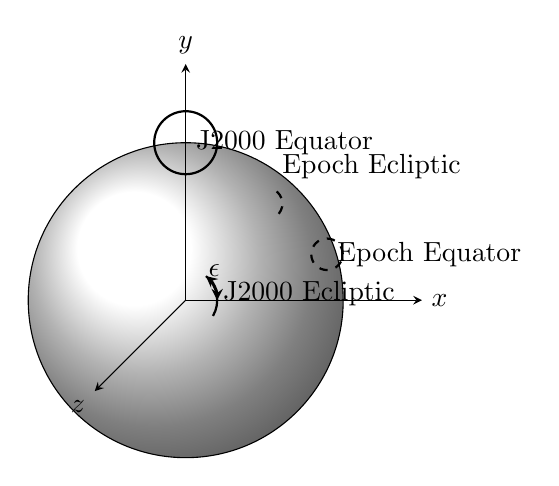
\begin{tikzpicture}[scale=2, >=stealth, line join=round]

  % Define the coordinates of the J2000 equator and ecliptic
  \coordinate (J2000-ecl) at (0,0,0);
  \coordinate (J2000-eq) at (0,1,0);

  % Define the coordinates of the epoch equator and ecliptic
  \coordinate (epoch-ecl) at (50:0.8);
  \coordinate (epoch-eq) at ($ (epoch-ecl) + (-40:0.5) $);

  % Define the radius of the sphere
  \pgfmathsetmacro\R{1}

  % Draw the sphere
  \draw[ball color=white] (0,0,0) circle[radius=\R];

  % Draw the J2000 equator and ecliptic
  \draw[thick] (J2000-eq) circle[radius=0.2*\R] node[right] {J2000 Equator};
  \draw[thick] (J2000-ecl) ++(50:0.2*\R) arc (50:-30:0.2*\R) node[above right] {J2000 Ecliptic};

  % Draw the epoch equator and ecliptic
  \draw[thick, dashed] (epoch-eq) circle[radius=0.1*\R] node[right] {Epoch Equator};
  \draw[thick, dashed] (epoch-ecl) ++(-40:0.1*\R) arc (-40:70:0.1*\R) node[above right] {Epoch Ecliptic};

  % Draw the celestial sphere axes
  \draw[->] (0,0,0) -- (1.5,0,0) node[right] {$x$};
  \draw[->] (0,0,0) -- (0,1.5,0) node[above] {$y$};
  \draw[->] (0,0,0) -- (0,0,1.5) node[below left] {$z$};

  % Label the angle between the two ecliptics
  \draw[<->,thick] ($(J2000-ecl) + (0.2,0,0)$) arc (0:50:0.2) node[midway,above] {$\epsilon$};

\end{tikzpicture}
\end{document}
